\documentclass[11pt, twoside, reqno]{book}
\usepackage{amssymb, amsthm, amsmath, amsfonts}
\usepackage{graphicx}
\usepackage{amsrefs}
\usepackage{color}
\usepackage{hyperref}
\usepackage{verbatim}
\usepackage[toc,page]{appendix}
\appendixpageoff

\usepackage{bardtex}

\styleoption{seniorproject}


\begin{document}

%For senior projects:
\titlepg{Mathematics is Fun}{Angela Albee}
    {May}{2099}

\abstr

The abstract should be brief, and non-technical.  Try to minimize the use of symbols in the abstract, so that you can use the abstract elsewhere.

\tableofcontents

\dedic

I dedicate this senior project to every person I have ever met in my life.

\acknowl

I would like to acknowledge the help I received from every person I have ever met in my life.

\startmain


\intro

Every senior project should have an introductory chapter that briefly summarizes or previews the content of the whole project.  The introductory chapter, which can be thought of as an expanded version of the abstract, is meant to give the big picture, and should include a discussion of the background to the project, place the project in the context of known results, and provide an informal summary of the main results.  Additionally, the introductory chapter should make clear what in the project is exposition of known results and what is original work.


\chapter{A Very Nice Chapter}
\label{chapA}

\section{An Even Nicer Section}
\label{secA1}

Before you state a theorem, it's best to give some intuitive idea of what the theorem is about.

\thm\label{thmAA} 
Let $\func fAB$ be a function.
%
\enum 
\item\label{thmAA1}
If $f$ has an inverse, then the inverse is unique.
%
\item\label{thmAA2}
If $f$ has a right inverse $g$ and a left inverse $h$, then $g = h$; hence $f$ has an inverse.
%
\item\label{thmAA3}
If $f$ has an inverse $g$, then $g$ has an inverse, which is $f$.
\eenum
\ethm
 
\demo
(\ref{thmAA1}). Suppose that $\func {g, h}BA$ are both inverses of $f$.  We will show that $g = h$.  By hypothesis on $g$ and $h$ we know, among other things, that $f \circ g = 1_B$ and $h \circ f = 1_A$.  Using a previous lemma we see that
%
\[
g  =  1_A \circ g  =  (h \circ f) \circ g  =  h \circ (f \circ g)  =  h \circ 1_B  =  h.
\]

\noindent (\ref{thmAA2}). The proof is virtually the same as in Part~(1).  
\smallskip

\noindent (\ref{thmAA3}).  Since $\func gBA$ is an inverse of $f$, then $g \circ f = 1_A$ and $f \circ g = 1_B$.  By the definition of inverses, it follows that $f$ is an inverse of $g$.  By Part~(1) of this theorem, we know that $f$ is the unique inverse of $g$.
\edemo


\section{The Best Section Ever}
\label{secA2}

Whenever possible, break up a long chapter into sections.

Also whenever possible, insert figures to aid the reader.  Always refer to the figures in the text.  We see the logo of the Mathematics Program at Bard in Figure~\ref{figMATHBARD}.

\begin{figure}[ht]
\centering
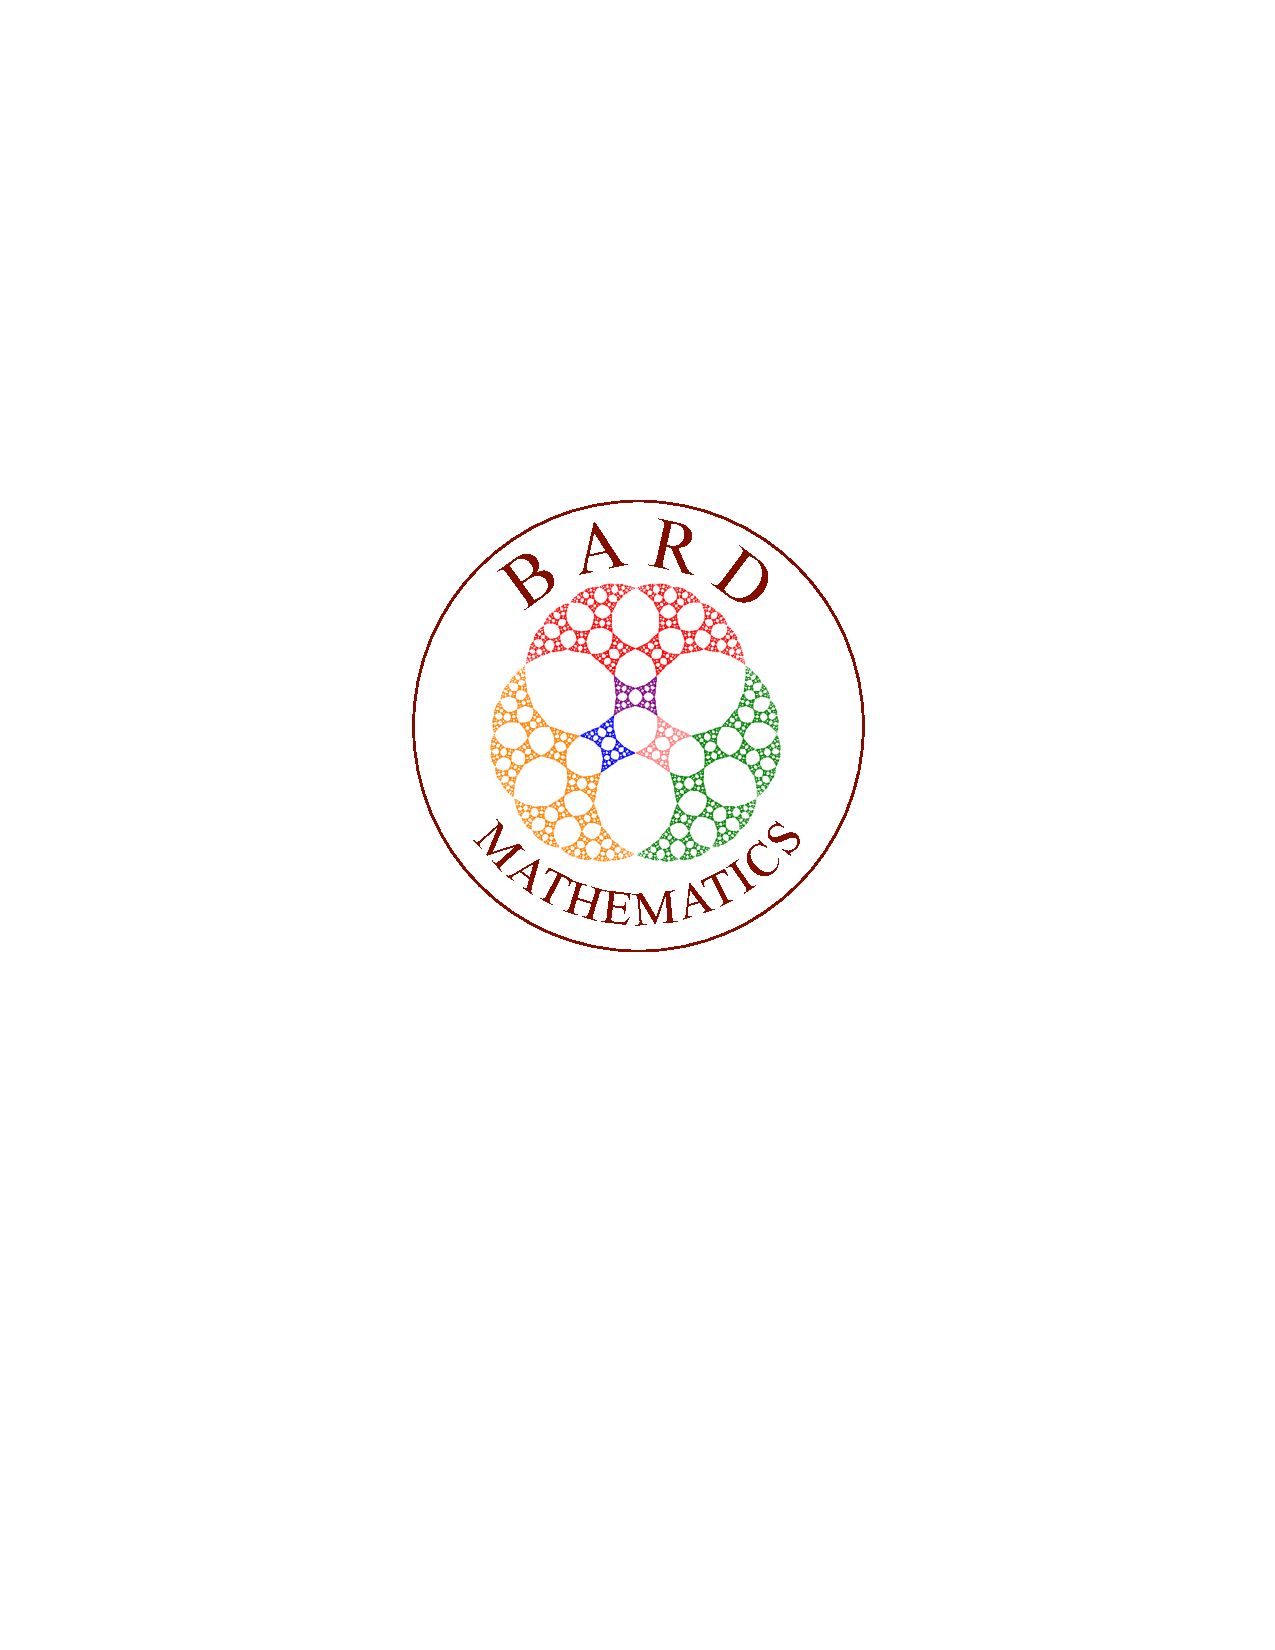
\includegraphics[scale=0.75]{math_prog_logo.pdf}
\caption{The Bard Mathematics Program Logo}
\label{figMATHBARD}
\end{figure}


\begin{appendices}
\chapter{I Like Appendices}

\section{A Lovely Appendix}

An appendix is very nice when you want to include some useful material that you don't want to put in the main text, in order to avoid disrupting the flow of your writing.  An appendix could contain background material, data, computer code and the like.

You can have as many appendices as you wish.

Each appendix is a chapter.  Each appendix can have sections if you wish.  If you put theorems and the like in an appendix, it should have sections, because otherwise the theorem numbering will have a $0$ for middle number.

You put theorems and the like in appendices exactly as you put them in the rest of the senior project.

\thm\label{thmAP} 
Let $\func fAB$ be a function.
%
\enum 
\item\label{thmAP1}
If $f$ has an inverse, then the inverse is unique.
%
\item\label{thmAP2}
If $f$ has a right inverse $g$ and a left inverse $h$, then $g = h$; hence $f$ has an inverse.
%
\item\label{thmAP3}
If $f$ has an inverse $g$, then $g$ has an inverse, which is $f$.
\eenum
\ethm
 
\demo
(\ref{thmAP1}). Suppose that $\func {g, h}BA$ are both inverses of $f$.  We will show that $g = h$.  By hypothesis on $g$ and $h$ we know, among other things, that $f \circ g = 1_B$ and $h \circ f = 1_A$.  Using a previous lemma we see that
%
\[
g  =  1_A \circ g  =  (h \circ f) \circ g  =  h \circ (f \circ g)  =  h \circ 1_B  =  h.
\]

\noindent (\ref{thmAP2}). The proof is virtually the same as in Part~(1).  
\smallskip

\noindent (\ref{thmAP3}).  Since $\func gBA$ is an inverse of $f$, then $g \circ f = 1_A$ and $f \circ g = 1_B$.  By the definition of inverses, it follows that $f$ is an inverse of $g$.  By Part~(1) of this theorem, we know that $f$ is the unique inverse of $g$.
\edemo

\end{appendices}


\begin{bibliog}

\bib{HOMOLOGY}{book}{
author = {Homology, Harold},
title = {Algebraic Topology for Dummies},
publisher = {Math Lights},
address = {Simplicialville, NY},
date = {2099}
}

\bib{CALCULUS}{article}{
author = {Calculus, Cathy},
title = {Why everyone should love calculus},
journal = {Journal of Fun Mathematics},
volume = {314},
date = {2099},
pages = {100--101}
}

\bib{PROJECT}{report}{
author = {Fractal, Fred},
author = {Graph, Germaine},
title = {How to Write a Great Senior Project in Mathematics},
eprint = {http://www.www.www.edu}
}

\end{bibliog}

\end{document}

% end of file bardproj_template.tex
